% Shared preamble for the multilayer-perceptron exercises.
% Each exercise is a standalone document: compile it from this directory.
\documentclass[11pt,a4paper]{article}

\usepackage[margin=2.35cm,top=1.85cm,bottom=2.15cm,headheight=22pt,headsep=9pt]{geometry}
\usepackage[T1]{fontenc}
\usepackage[utf8]{inputenc}
\usepackage[english]{babel}
\usepackage{lmodern}
\usepackage{textcomp}
\usepackage{microtype}
\usepackage{amsmath,amssymb,amsthm,mathtools}
\usepackage{booktabs}
\usepackage{array}
\usepackage{enumitem}
\usepackage{xcolor}
\usepackage{tikz}
\usetikzlibrary{arrows.meta,positioning,calc}
\usepackage{pgfplots}
\pgfplotsset{compat=1.17}
\usepackage[hypcap=false]{caption}
\usepackage{needspace}
\usepackage{titlesec}
\usepackage{fancyhdr}
\usepackage[hidelinks,unicode]{hyperref}

\setlength{\parindent}{1.15em}
\setlength{\parskip}{0pt}
\setlength{\abovedisplayskip}{7pt plus 2pt minus 2pt}
\setlength{\belowdisplayskip}{7pt plus 2pt minus 2pt}
\setlength{\abovedisplayshortskip}{4pt plus 2pt}
\setlength{\belowdisplayshortskip}{5pt plus 2pt}
\setlength{\emergencystretch}{2em}
\allowdisplaybreaks[1]

\definecolor{navy}{HTML}{1B365D}
\definecolor{ink}{HTML}{1C1917}
\definecolor{rulegold}{HTML}{8C6A32}
\definecolor{wash}{HTML}{F6F3EC}
\definecolor{accent}{HTML}{7A2E2E}

\pagestyle{fancy}
\fancyhf{}
\fancyhead[L]{\small\sffamily\color{navy}Universidad Pontificia Comillas}
\fancyhead[R]{\small\sffamily\color{navy}\exerciseshort}
\fancyfoot[C]{\small\color{ink!70}\thepage}
\renewcommand{\headrulewidth}{0.4pt}
\renewcommand{\headrule}{%
  \hbox to\headwidth{\color{rulegold}\leaders\hrule height \headrulewidth\hfill}%
}
\fancypagestyle{plain}{%
  \fancyhf{}%
  \fancyfoot[C]{\small\color{ink!70}\thepage}%
  \renewcommand{\headrulewidth}{0pt}%
}

\captionsetup{
  font={small},
  labelfont={sf,bf,color=navy},
  labelsep=period,
  skip=7pt
}

\titleformat{\section}
  {\Large\bfseries\sffamily\color{navy}}
  {\thesection}{0.55em}{}
  [\vspace{0.2em}{\color{navy}\titlerule[0.55pt]}]
\titleformat{\subsection}
  {\normalsize\bfseries\sffamily\color{navy}}
  {}{0pt}{}
  [\vspace{-0.15em}{\color{rulegold}\titlerule[0.4pt]}]
\titlespacing*{\section}{0pt}{1.15em}{0.55em}
\titlespacing*{\subsection}{0pt}{1.05em}{0.4em}

\theoremstyle{plain}
\newtheorem{lemma}{Lemma}
\newtheorem{proposition}{Proposition}
\theoremstyle{definition}
\newtheorem*{remark}{Remark}

\setlist[enumerate]{leftmargin=1.7em,itemsep=0.5em,topsep=0.35em,labelsep=0.5em}
\setlist[itemize]{leftmargin=1.35em,itemsep=0.25em,topsep=0.3em}

\newcommand{\exerciseshort}{Multilayer perceptrons}
\newcommand{\R}{\mathbb{R}}
\newcommand{\E}{\mathbb{E}}
\DeclareMathOperator{\Var}{Var}
\DeclareMathOperator{\relu}{ReLU}
\DeclarePairedDelimiter{\abs}{\lvert}{\rvert}
\DeclarePairedDelimiter{\norm}{\lVert}{\rVert}
\newcommand{\dd}{\mathrm{d}}
\newcommand{\T}{\mathsf{T}}

\tikzset{
  neuron/.style={
    circle, draw=navy, line width=0.65pt, minimum size=8.2mm,
    inner sep=0pt, font=\small, fill=white
  },
  ninput/.style={neuron, fill=navy!6},
  nhidden/.style={neuron, fill=navy!11},
  noutput/.style={neuron, fill=rulegold!18},
  ndead/.style={neuron, fill=ink!8, draw=ink!45, text=ink!55},
  nedge/.style={
    -{Stealth[length=1.65mm,width=1.35mm]},
    draw=ink!72, line width=0.45pt
  },
  ntag/.style={font=\scriptsize\sffamily, text=navy}
}

% #1 number, #2 running head, #3 display title, #4 introductory paragraph
\newcommand{\exercisefront}[4]{%
  \thispagestyle{plain}%
  \gdef\exerciseshort{Exercise #1\enspace\textperiodcentered\enspace #2}%
  \noindent{\sffamily\footnotesize\color{navy}%
    \MakeUppercase{Universidad Pontificia Comillas}}\par
  \vspace{0.15em}
  \noindent{\sffamily\footnotesize\color{ink!80}%
    Teaching collection of Eduardo C\'esar Garrido Merch\'an}\par
  \vspace{0.55em}
  \noindent{\sffamily\small\color{ink!75}%
    Multilayer perceptrons%
    \enspace\textcolor{rulegold}{\textperiodcentered}\enspace
    Exercise #1 of 3}\par
  \vspace{0.7em}
  \noindent{\sffamily\LARGE\bfseries\color{navy}#3\par}
  \vspace{0.35em}
  \noindent{\color{rulegold}\rule{\textwidth}{0.7pt}}\par
  \vspace{0.75em}
  \noindent #4\par
  \vspace{0.15em}
}

\newcommand{\solutionpart}[1]{%
  \Needspace{8\baselineskip}%
  \subsection*{Solution to (#1)}%
}

\hypersetup{
  pdfauthor={Eduardo C\'esar Garrido Merch\'an},
  pdfsubject={Graduate exercises on multilayer perceptrons}
}

\hypersetup{pdftitle={Exercise 3. Initialization, vanishing gradients, and regularization}}

\begin{document}

\exercisefront{3}{Optimization}
  {Initialization, vanishing gradients, and regularization}
  {Training a multilayer perceptron is a nonconvex optimization problem. The questions below isolate three mechanisms that decide whether that optimization moves: the scale of the random initial weights, the product of derivatives along a deep sigmoid chain, and the effect of an \(\ell_2\) penalty or of dropout. Each identity is proved from the definitions. The numerical parts are small linear systems and one fully explicit back-propagation of depth four.}

\section{Setup}

The logistic sigmoid \(\sigma(t)=(1+e^{-t})^{-1}\) has derivative \(\sigma'(t)=\sigma(t)\bigl(1-\sigma(t)\bigr)\). The rectified linear unit is \(\relu(t)=\max\{t,0\}\). An empirical loss written \(L\) is a mean over the training sample unless a question says otherwise. Weights of a layer with \(n_{\mathrm{in}}\) inputs and \(n_{\mathrm{out}}\) outputs form a matrix in \(\R^{n_{\mathrm{out}}\times n_{\mathrm{in}}}\).

\section{Questions}

\begin{enumerate}[label=\textbf{(\alph*)}]
  \item Consider a single linear layer \(y = Wx\), with the entries of \(W\) drawn i.i.d.\ with mean \(0\) and variance \(\sigma_w^2\), independently of \(x\). Assume the coordinates of \(x\in\R^{n_{\mathrm{in}}}\) are i.i.d.\ with mean \(0\) and variance \(\sigma_x^2\). Derive \(\Var(y_i)\). Next let \(g=\partial L/\partial y\in\R^{n_{\mathrm{out}}}\) have i.i.d.\ coordinates of mean \(0\) and variance \(\sigma_g^2\), independent of \(W\), and derive \(\Var\bigl((W^\T g)_j\bigr)\). The two requirements \(\Var(y_i)=\sigma_x^2\) and \(\Var\bigl((W^\T g)_j\bigr)=\sigma_g^2\) prescribe two different values of \(\sigma_w^2\). Show that the Glorot (Xavier) choice
  \[
    \sigma_w^2 = \frac{2}{n_{\mathrm{in}}+n_{\mathrm{out}}}
  \]
  is the harmonic mean of those two values, and compute it numerically for \(n_{\mathrm{in}}=256\), \(n_{\mathrm{out}}=128\). State which hypothesis fails if the input coordinates have a nonzero mean.

  \item Let \(Z\sim\mathcal N(0,\tau^2)\) and \(R=\relu(Z)\). Derive \(\E[R]\), \(\E[R^2]\), and \(\Var(R)\) in closed form. Then consider a layer \(z = Wh\) followed by a coordinatewise ReLU, with weights that are i.i.d., symmetric about \(0\), of variance \(\sigma_w^2\), and independent of \(h\). Prove that each preactivation is symmetric about \(0\), and that the second moment of a ReLU output equals \(\tfrac12 n_{\mathrm{in}}\sigma_w^2\) times the common second moment of the incoming coordinates, assuming those second moments exist and are equal. Deduce the He initialisation \(\sigma_w^2 = 2/n_{\mathrm{in}}\). For the same fan-in and fan-out as in part~(a), compute the He standard deviation and compare it with the Glorot value. Explain what the He rule preserves, and what it does not preserve.

  \item Prove that \(0 < \sigma'(t) \le 1/4\) for every real \(t\), with equality only at \(t=0\). Consider a width-\(1\) sigmoid chain of length \(L\),
  \[
    a_0 = x,
    \qquad
    z_\ell = w_\ell a_{\ell-1} + b_\ell,
    \qquad
    a_\ell = \sigma(z_\ell),
    \qquad
    L_{\mathrm{sq}} = \tfrac12(a_L-y)^2.
  \]
  Derive \(\partial L_{\mathrm{sq}}/\partial w_1\) as an explicit product. Deduce a bound under the additional assumption \(\abs{w_\ell}\le 1\) and \(y\in[0,1]\). Then specialise to \(L=4\), \(w_\ell=1\), \(b_\ell=0\), \(x=2\), \(y=1\): compute the forward activations, the back-propagated deltas, and \(\partial L_{\mathrm{sq}}/\partial w_\ell\) for each layer, to six decimals. Separately, evaluate \((1/4)^L\) and \(\sigma'(2)^L\) at \(L=1,2,10\).

  Finally, prove the dying-ReLU lemma. If a hidden unit has preactivation \(w^\T a(x_n)+b < 0\) at every training point, then under gradient descent with no momentum that unit's parameters never move, and the unit remains inactive on the whole training set.

  \item Let \(S(W)\) be a differentiable data-fit term and let
  \[
    L_\lambda(W) = S(W) + \frac{\lambda}{2}\norm{W}_F^2, \qquad \lambda>0.
  \]
  Derive \(\nabla L_\lambda\) and the gradient-descent update. Show that the update is identical to weight decay, \(W\leftarrow (1-\eta\lambda)W - \eta\nabla S(W)\), and state briefly why the identity does not survive the adaptive scaling used by Adam. Interpreting \(S\) as a mean negative log-likelihood and the weights as a priori independent \(\mathcal N(0,\sigma_p^2)\) variables, identify \(\lambda\) in terms of \(\sigma_p^2\) and the sample size \(N\).

  For a concrete ridge problem, let
  \[
    A
    =
    \begin{pmatrix} 1 & 99/100 \\ 99/100 & 1 \end{pmatrix},
    \qquad
    c = \begin{pmatrix} 1 \\ -1 \end{pmatrix},
  \]
  and solve \(Aw=c\) together with \((A+I)w=c\). Compute both Euclidean norms and both condition numbers. A short route is to notice that \(c\) is an eigenvector of \(A\).

  \item Inverted dropout with keep probability \(p\in(0,1]\) replaces a vector \(h\) by \(\tilde h_j = m_j h_j/p\), where the \(m_j\) are i.i.d.\ Bernoulli\((p)\) and independent of \(h\). Prove that \(\E[\tilde h\mid h] = h\), so the deterministic network evaluated at test time needs no extra rescaling. Then restrict to a linear predictor \(\hat y = w^\T\tilde x\) and the squared loss on one pair \((x,y)\). Prove
  \begin{equation}
    \E\bigl[(y-w^\T\tilde x)^2 \bigm| x,y\bigr]
    =
    \bigl(y-w^\T x\bigr)^2
    + \frac{1-p}{p}\sum_{j=1}^{d} x_j^2 w_j^2.
    \label{eq:dropout-identity}
  \end{equation}
  Check the identity by enumerating all four masks for \(p=1/2\), \(x=(2,1)^\T\), \(w=(1,1)^\T\), and \(y=0\). Explain in what sense this is an \(\ell_2\) penalty, and what the identity does not say about dropout inside a multilayer perceptron.
\end{enumerate}

The worked solution begins on the next page.

\clearpage
\section{Solutions}

\solutionpart{a}

Expand the \(i\)th output coordinate as \(y_i = \sum_{j=1}^{n_{\mathrm{in}}} W_{ij} x_j\). Independence of distinct weights, and independence of the weights from \(x\), kill the cross terms once the weights are centred: if \(j\neq k\), then \(\E[W_{ij}W_{ik}]=0\), so
\[
  \Var(y_i)
  =
  \sum_{j=1}^{n_{\mathrm{in}}} \E[W_{ij}^2]\,\E[x_j^2]
  =
  n_{\mathrm{in}}\,\sigma_w^2\,\sigma_x^2.
\]
The passage from \(\E[x_j^2]\) to \(\sigma_x^2\) uses \(\E[x_j]=0\). The same expansion for the backward signal \(u = W^\T g\), whose \(j\)th coordinate sums \(n_{\mathrm{out}}\) products \(W_{ij} g_i\), gives
\[
  \Var(u_j) = n_{\mathrm{out}}\,\sigma_w^2\,\sigma_g^2.
\]
Preserving the forward variance means \(n_{\mathrm{in}}\sigma_w^2 = 1\). Preserving the backward variance means \(n_{\mathrm{out}}\sigma_w^2 = 1\). These constraints agree only for square layers. The harmonic mean of the two admissible variances \(1/n_{\mathrm{in}}\) and \(1/n_{\mathrm{out}}\) is
\[
  \frac{2}{\,1/(1/n_{\mathrm{in}}) + 1/(1/n_{\mathrm{out}})\,}
  =
  \frac{2}{n_{\mathrm{in}}+n_{\mathrm{out}}},
\]
which is the Glorot variance. For \(n_{\mathrm{in}}=256\) and \(n_{\mathrm{out}}=128\),
\[
  \sigma_w^2 = \frac{2}{384} = \frac{1}{192},
  \qquad
  \sigma_w = \frac{1}{\sqrt{192}} = \frac{\sqrt{3}}{24} \approx 0.072169.
\]
The derivation linearises the layer: an activation with slope \(1\) at the operating point, such as \(\tanh\) near the origin, is covered, whereas a sigmoid is not, because \(\sigma'(0)=1/4\). Part~(c) measures that extra contraction.

If \(\E[x_j]\) is not zero, centred weights still give \(\E[y_i]=0\), but
\[
  \E[y_i^2]
  =
  n_{\mathrm{in}}\sigma_w^2\,\E[x_1^2]
  =
  n_{\mathrm{in}}\sigma_w^2\bigl(\sigma_x^2 + (\E x_1)^2\bigr).
\]
The output variance then exceeds \(n_{\mathrm{in}}\sigma_w^2\sigma_x^2\). Glorot's balance of variances uses the zero-mean hypothesis in an essential way. Preserving second moments rather than variances would replace \(\sigma_x^2\) by \(\E[x_1^2]\) and would stay valid without that hypothesis.

\solutionpart{b}

The density of \(Z\) is \((\tau\sqrt{2\pi})^{-1}\exp\bigl(-z^2/(2\tau^2)\bigr)\). For the mean of the rectified variable, substitute \(z=\tau u\):
\begin{align*}
  \E[R]
  &=
  \int_0^\infty z\cdot\frac{1}{\tau\sqrt{2\pi}}
  \exp\Bigl(-\frac{z^2}{2\tau^2}\Bigr)\,\dd z
  =
  \tau\int_0^\infty u\cdot\frac{1}{\sqrt{2\pi}}\,e^{-u^2/2}\,\dd u.
\end{align*}
The remaining integral equals \(1/\sqrt{2\pi}\), because \(\int_0^\infty u e^{-u^2/2}\,\dd u = 1\). Hence
\[
  \E[R] = \frac{\tau}{\sqrt{2\pi}}.
\]
For the second moment, symmetry of \(z\mapsto z^2\) about the origin cuts the Gaussian integral in half:
\[
  \E[R^2]
  =
  \int_0^\infty z^2\cdot\frac{1}{\tau\sqrt{2\pi}}
  \exp\Bigl(-\frac{z^2}{2\tau^2}\Bigr)\,\dd z
  =
  \tfrac12\E[Z^2]
  =
  \frac{\tau^2}{2}.
\]
Therefore
\[
  \Var(R)
  =
  \frac{\tau^2}{2} - \frac{\tau^2}{2\pi}
  =
  \tau^2\cdot\frac{\pi-1}{2\pi}.
\]
The factor \((\pi-1)/(2\pi)\) is about \(0.3408\), strictly smaller than the second moment \(\tau^2/2\). Rectification both discards mass and shifts the mean.

Now let \(z_i = \sum_{j=1}^{n_{\mathrm{in}}} W_{ij} h_j\), with the \(W_{ij}\) i.i.d., independent of \(h\), and symmetric about \(0\). Replacing \(W\) by \(-W\) does not change the law of \(W\) and leaves \(h\) fixed, so \(z_i\) and \(-z_i\) are equal in law. In particular \(\E[z_i]=0\) whenever the expectation exists. Symmetry alone, with no Gaussian assumption, yields \(\E[\relu(z_i)^2] = \tfrac12\E[z_i^2]\): the integrand \(z^2\) puts equal mass on the positive and negative halves.

Expanding the second moment and using independence,
\[
  \E[z_i^2]
  =
  \sum_{j=1}^{n_{\mathrm{in}}} \E[W_{ij}^2]\,\E[h_j^2]
  =
  \sigma_w^2\sum_{j=1}^{n_{\mathrm{in}}}\E[h_j^2],
\]
the cross terms vanishing because \(\E[W_{ij}W_{ik}]=0\) for \(j\neq k\). If every incoming coordinate has the same second moment \(v\), then \(\E[\relu(z_i)^2] = \tfrac12 n_{\mathrm{in}}\sigma_w^2\, v\). Asking this to equal \(v\), for \(v>0\), forces
\[
  \sigma_w^2 = \frac{2}{n_{\mathrm{in}}}.
\]
That is the He initialisation. It preserves the second moment of the activations across a ReLU layer. It does not preserve the mean: even if the incoming coordinates were centred, symmetry of the weights makes the preactivations centred, and the calculation above then shifts the mean of each ReLU output to a positive value. It also does not preserve the variance, which is the second moment minus the square of that new mean. For a Gaussian preactivation of variance \(\tau^2\), the variance after ReLU is \(\tau^2(\pi-1)/(2\pi)\) rather than \(\tau^2/2\). The rule is still the standard way to keep the scale of \(h\) from exploding or collapsing with depth; the residual mean shift is one reason later architectures add normalisation.

For \(n_{\mathrm{in}}=256\), the He standard deviation is
\[
  \sigma_w = \sqrt{\frac{2}{256}} = \frac{1}{\sqrt{128}} = \frac{\sqrt{2}}{16} \approx 0.088388,
\]
against the Glorot value \(0.072169\). The He weights are larger by a factor \(\sqrt{2\cdot 192/256} = \sqrt{3/2}\approx 1.2247\), which is the correction for discarding, in the second-moment sense, half of the preactivation.

\solutionpart{c}

Set \(u=\sigma(t)\in(0,1)\). Then \(\sigma'(t)=u(1-u)\). The quadratic \(u(1-u)\) on \((0,1)\) opens downwards and has its unique maximum at \(u=1/2\), where its value is \(1/4\). Since \(u=1/2\) occurs only at \(t=0\), one has \(0<\sigma'(t)\le 1/4\), with equality only at the origin. The inequality is strict as soon as the preactivation leaves \(0\): \(\sigma'(2)=\sigma(2)\bigl(1-\sigma(2)\bigr)\). With \(\sigma(2)=(1+e^{-2})^{-1}=0.880797\),
\[
  \sigma'(2) = 0.104994,
\]
a little under half of the maximum.

For the width-\(1\) chain, write \(\delta_\ell = \partial L_{\mathrm{sq}}/\partial z_\ell\). The output factor is \(\delta_L = (a_L-y)\sigma'(z_L)\). Differentiating \(z_{\ell+1} = w_{\ell+1}a_\ell + b_{\ell+1}\) and \(a_\ell=\sigma(z_\ell)\) gives the recurrence \(\delta_\ell = \delta_{\ell+1}\, w_{\ell+1}\, \sigma'(z_\ell)\), hence
\begin{equation}
  \delta_1
  =
  (a_L-y)\,\sigma'(z_L)\prod_{\ell=1}^{L-1}\bigl(w_{\ell+1}\,\sigma'(z_\ell)\bigr)
  \label{eq:delta-prod}
\end{equation}
and, because \(\partial z_1/\partial w_1 = a_0 = x\),
\[
  \frac{\partial L_{\mathrm{sq}}}{\partial w_1}
  =
  (a_L-y)\,\sigma'(z_L)
  \Biggl(\prod_{\ell=1}^{L-1} w_{\ell+1}\,\sigma'(z_\ell)\Biggr) x.
\]
There are \(L\) factors of a sigmoid derivative in this product once \(\sigma'(z_L)\) is counted. Under \(\abs{w_\ell}\le 1\) and \(y\in[0,1]\) one has \(\abs{a_L-y}\le 1\), so
\begin{equation}
  \Biggl\lvert\frac{\partial L_{\mathrm{sq}}}{\partial w_1}\Biggr\rvert
  \le
  \frac{\abs{x}}{4^L}.
  \label{eq:vanish-bound}
\end{equation}
The bound is a product of local contractions. It does not require the weights to be small: \(\abs{w_\ell}\le 1\) is enough, and equality in the derivative bound would demand every preactivation to sit at \(0\), which is incompatible with a nonzero signal travelling down the chain. Table~\ref{tab:powers} records the pure products. At depth \(10\), even the most favourable factor \((1/4)^{10} = 2^{-20} = 1/1\,048\,576 \approx 9.537\times 10^{-7}\) has wiped out six orders of magnitude, and the saturated factor \(\sigma'(2)^{10}\approx 1.628\times 10^{-10}\) has wiped out ten.

\begin{center}
\captionof{table}{Products of the largest sigmoid slope and of the slope at preactivation \(2\).}
\label{tab:powers}
\vspace{0.4em}
\begin{tabular}{@{}rrr@{}}
\toprule
\(L\) & \((1/4)^L\) & \(\sigma'(2)^L\) \\
\midrule
\(1\)  & \(2.500\times 10^{-1}\) & \(1.050\times 10^{-1}\) \\
\(2\)  & \(6.250\times 10^{-2}\) & \(1.102\times 10^{-2}\) \\
\(10\) & \(9.537\times 10^{-7}\) & \(1.628\times 10^{-10}\) \\
\bottomrule
\end{tabular}
\end{center}

For the concrete chain, \(b_\ell=0\) and \(w_\ell=1\), so \(z_1=x=2\) and \(z_{\ell+1}=a_\ell=\sigma(z_\ell)\). Six-decimal evaluation gives the forward pass
\begin{align*}
  z_1 &= 2,        & a_1 &= 0.880797, & \sigma'(z_1) &= 0.104994,\\
  z_2 &= 0.880797, & a_2 &= 0.706987, & \sigma'(z_2) &= 0.207156,\\
  z_3 &= 0.706987, & a_3 &= 0.669735, & \sigma'(z_3) &= 0.221190,\\
  z_4 &= 0.669735, & a_4 &= 0.661444, & \sigma'(z_4) &= 0.223936.
\end{align*}
The loss is \(\tfrac12(0.661444-1)^2 = 0.057310\). Back-propagation starts at
\[
  \delta_4 = (a_4-1)\sigma'(z_4) = -0.075815
\]
and applies \(\delta_\ell = \delta_{\ell+1}\,\sigma'(z_\ell)\), since every weight equals \(1\):
\[
  \delta_3 = -0.016769,
  \qquad
  \delta_2 = -0.003474,
  \qquad
  \delta_1 = -0.000365.
\]
Multiplying by the incoming activation, \(\partial L_{\mathrm{sq}}/\partial w_\ell = \delta_\ell\, a_{\ell-1}\) with \(a_0=2\), produces
\begin{equation*}
\begin{aligned}
  \partial L_{\mathrm{sq}}/\partial w_1 &= -0.000729, &
  \partial L_{\mathrm{sq}}/\partial w_2 &= -0.003060,\\
  \partial L_{\mathrm{sq}}/\partial w_3 &= -0.011856, &
  \partial L_{\mathrm{sq}}/\partial w_4 &= -0.050776.
\end{aligned}
\end{equation*}
The gradient at the first weight is smaller than the gradient at the last weight by a factor of about \(69.6\). Figure~\ref{fig:chain} is this chain. Nothing in the algebra has overflowed or underflowed; the decay is the product of four ordinary derivatives, each at most \(1/4\), and here each is near \(0.2\) after the first saturated step. ReLU removes this particular mechanism, because its derivative on the positive ray is \(1\), but it introduces a different degeneracy, proved next.

\begin{center}
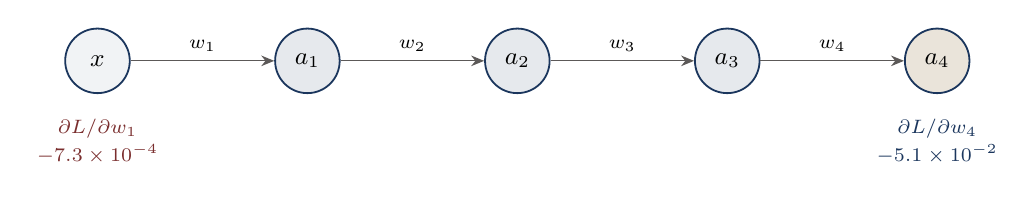
\begin{tikzpicture}[x=1.72cm]
  \node[ninput] (a0) at (0,0) {$x$};
  \node[nhidden] (a1) at (1.55,0) {$a_1$};
  \node[nhidden] (a2) at (3.1,0) {$a_2$};
  \node[nhidden] (a3) at (4.65,0) {$a_3$};
  \node[noutput] (a4) at (6.2,0) {$a_4$};
  \draw[nedge] (a0) -- (a1) node[midway, above, font=\scriptsize] {$w_1$};
  \draw[nedge] (a1) -- (a2) node[midway, above, font=\scriptsize] {$w_2$};
  \draw[nedge] (a2) -- (a3) node[midway, above, font=\scriptsize] {$w_3$};
  \draw[nedge] (a3) -- (a4) node[midway, above, font=\scriptsize] {$w_4$};
  \node[font=\scriptsize, align=center, text=accent, anchor=north] at (0,-0.62)
    {$\partial L/\partial w_1$\\[1pt] $-7.3\times 10^{-4}$};
  \node[font=\scriptsize, align=center, text=navy, anchor=north] at (6.2,-0.62)
    {$\partial L/\partial w_4$\\[1pt] $-5.1\times 10^{-2}$};
\end{tikzpicture}
\captionof{figure}{Width-\(1\) sigmoid chain. With unit weights, zero biases, and input \(2\), the loss derivative at \(w_1\) is about seventy times smaller than the derivative at \(w_4\).}
\label{fig:chain}
\end{center}

\paragraph{Dying ReLUs.}
Let a hidden unit compute \(z(x) = w^\T a(x)+b\) and contribute \(\relu(z(x))\) to the next layer. Suppose \(z(x_n)<0\) for every training index \(n\). The training set is finite, so the strict inequalities \(z(x_n)<0\) leave a common open neighbourhood of the current \((w,b)\) on which every training preactivation stays negative. On that neighbourhood \(\relu(z(x_n))\) is constant in the parameters. The training loss, being a function of these outputs and of the other units, has partial derivatives \(0\) with respect to this \(w\) and this \(b\). A gradient step of any size therefore leaves the pair \((w,b)\) exactly where it is. The preactivations on the training set do not change, the strict inequalities persist, and the unit never becomes active on that set.

The same conclusion holds for minibatch stochastic gradient descent: every minibatch is drawn from a set on which the unit is inactive, so every stochastic gradient in these parameters is zero. The argument uses plain gradient steps. A momentum buffer that was already nonzero could still move the weights; the lemma does not claim otherwise. The boundary case \(z(x_n)\le 0\), with the conventional choice \(\relu'(0)=0\), gives the same zero gradient. He initialisation does not remove the lemma. It only keeps preactivations from starting at a tiny scale, so that a unit is less likely to lie strictly on the negative side of every training point at step zero.

\solutionpart{d}

The Frobenius inner product satisfies \(\dd\bigl(\tfrac12\norm{W}_F^2\bigr) = \langle W, \dd W\rangle_F\), so \(\nabla(\tfrac12\norm{W}_F^2) = W\) and
\[
  \nabla L_\lambda(W) = \nabla S(W) + \lambda W.
\]
One gradient step of size \(\eta>0\) is
\begin{align}
  W^{+}
  &= W - \eta\bigl(\nabla S(W)+\lambda W\bigr) \nonumber\\
  &= (1-\eta\lambda)\,W - \eta\,\nabla S(W).
  \label{eq:weightdecay}
\end{align}
The second line is weight decay: shrink the current weights by the factor \(1-\eta\lambda\), then apply the usual step on the unregularised gradient. For stochastic gradient descent the two implementations are algebraically identical.

Adam applies a diagonal preconditioner, built from moving averages of the gradient and of its square, to whatever vector it is given as ``the gradient.'' If the \(\ell_2\) term is folded into the loss, that preconditioner scales \(\nabla S(W)+\lambda W\), and the penalty is attenuated in coordinates where the preconditioner is small. Decoupled weight decay applies the factor \((1-\eta\lambda)\) directly to \(W\), as in \eqref{eq:weightdecay}, and sends only \(\nabla S(W)\) through the preconditioner. Those two maps differ. Loshchilov and Hutter (2019) isolate the difference and recommend the decoupled form.

For the Bayesian reading, let \(S(w) = -N^{-1}\sum_{n=1}^N \log p(y_n\mid x_n,w)\) be a mean negative log-likelihood, and let the coordinates of \(w\) be i.i.d.\ \(\mathcal N(0,\sigma_p^2)\) a priori. The negative log prior contributes \(\norm{w}_2^2/(2\sigma_p^2)\), up to an additive constant. Dividing the whole posterior objective by \(N\) so that it matches the mean likelihood term produces
\[
  S(w) + \frac{1}{2N\sigma_p^2}\,\norm{w}_2^2.
\]
Comparison with \(L_\lambda\) gives \(\lambda = 1/(N\sigma_p^2)\). Using a sum of negative log-likelihoods instead of a mean would omit the factor \(1/N\). The Gaussian prior is isotropic: every coordinate is pulled toward \(0\) with the same coefficient. Part~(e) produces a penalty that does not have this symmetry.

\paragraph{The ridge system.}
The eigenvalues of a matrix \(\bigl(\begin{smallmatrix} 1 & \rho\\ \rho & 1\end{smallmatrix}\bigr)\) are \(1\pm\rho\), with eigenvectors \((1,1)^\T\) and \((1,-1)^\T\). Here \(\rho=99/100\), so
\[
  \lambda_{\max}(A) = \frac{199}{100},
  \qquad
  \lambda_{\min}(A) = \frac{1}{100},
  \qquad
  \kappa_2(A) = 199.
\]
The matrix is symmetric positive definite, hence a legitimate Gram matrix \(X^\T X\). The right-hand side \(c=(1,-1)^\T\) is an eigenvector for \(\lambda_{\min}\):
\[
  A c = \frac{1}{100}\, c,
  \qquad
  A(100\, c) = c.
\]
The unregularised solution is therefore \(w_{\mathrm{ols}} = (100,\,-100)^\T\), with
\[
  \norm{w_{\mathrm{ols}}}_2 = 100\sqrt{2}.
\]
Adding the identity shifts every eigenvalue by \(1\), so
\[
  \lambda_{\max}(A+I) = \frac{299}{100},
  \qquad
  \lambda_{\min}(A+I) = \frac{101}{100},
  \qquad
  \kappa_2(A+I) = \frac{299}{101} \approx 2.960.
\]
Along the same eigenvector, \((A+I)c = (101/100)\, c\), and
\[
  w_{\lambda}
  =
  \frac{100}{101}\, c
  =
  \begin{pmatrix} 100/101 \\ -100/101 \end{pmatrix},
  \qquad
  \norm{w_{\lambda}}_2 = \frac{100}{101}\sqrt{2}.
\]
Regularisation divides this particular solution by \(101\). The mechanism is visible in the scalar formula for one eigen-coordinate, \(1/(\lambda_{\min}+\lambda)\) against \(1/\lambda_{\min}\): the ridge term dominates the tiny eigenvalue \(1/100\), while it barely moves the eigenvalue \(199/100\). The condition number falls from \(199\) to \(299/101\). The fit term that produced \(c\) was deliberately aligned with the ill-conditioned direction; a right-hand side parallel to \((1,1)^\T\) would have been stable already, and the same \(\lambda\) would have changed it only by the modest factor \((199/100)/(299/100)=199/299\).

\solutionpart{e}

Condition on \(h\). For each coordinate, \(\E[m_j]=p\), so \(\E[m_j h_j/p \mid h] = h_j\). Coordinates separate, and \(\E[\tilde h\mid h]=h\). The test-time forward pass can therefore use the original vector \(h\). The factor \(1/p\) has already made the training-time estimator unbiased. The original dropout convention omits that factor during training and multiplies the outgoing weights by \(p\) at test time; the two conventions implement the same mean network.

For the squared loss, expand the residual about the unmasked prediction:
\[
  y - w^\T\tilde x
  =
  \bigl(y-w^\T x\bigr) + w^\T(x-\tilde x).
\]
The cross term has conditional expectation zero because \(\E[\tilde x\mid x] = x\). Independence of the masks makes the coordinates of \(x-\tilde x\) uncorrelated. Indeed
\[
  x_j-\tilde x_j = x_j\Bigl(1-\frac{m_j}{p}\Bigr),
  \qquad
  \Var\Bigl(\frac{m_j}{p}\Bigr)
  =
  \frac{1}{p^2}\cdot p(1-p)
  =
  \frac{1-p}{p},
\]
and therefore
\begin{align*}
  \E\bigl[\bigl(w^\T(x-\tilde x)\bigr)^2 \bigm| x\bigr]
  &=
  \sum_{j=1}^{d} w_j^2 x_j^2\cdot\Var\Bigl(\frac{m_j}{p}\Bigr)
  =
  \frac{1-p}{p}\sum_{j=1}^{d} x_j^2 w_j^2.
\end{align*}
Adding the squared bias term \((y-w^\T x)^2\) is \eqref{eq:dropout-identity}. Averaging over a training sample replaces the single-example penalty by
\[
  \frac{1-p}{p}\sum_{j=1}^{d}\hat s_j\, w_j^2,
  \qquad
  \hat s_j = \frac1N\sum_{n=1}^N x_{nj}^2.
\]
This is an \(\ell_2\) penalty whose coefficient on \(w_j\) is proportional to the empirical second moment of feature \(j\). It is diagonal in the coordinate basis, and it is not the isotropic penalty \((\lambda/2)\norm{w}_2^2\) of part~(d) unless all features happen to have the same second moment. Large coordinates are regularised more than small ones.

The numerical check uses \(p=1/2\), so \((1-p)/p=1\) and \(\tilde x_j = 2 m_j x_j\). The unmasked prediction is \(w^\T x = 3\), the squared residual is \(9\), and the penalty is \(x_1^2 w_1^2 + x_2^2 w_2^2 = 4+1 = 5\). The identity predicts conditional expected loss \(14\). The four masks, each of probability \(1/4\), give
\begin{center}
\begin{tabular}{@{}cccc@{}}
\toprule
\((m_1,m_2)\) & \(\tilde x\) & prediction & squared loss \\
\midrule
\((0,0)\) & \((0,0)\) & \(0\) & \(0\) \\
\((0,1)\) & \((0,2)\) & \(2\) & \(4\) \\
\((1,0)\) & \((4,0)\) & \(4\) & \(16\) \\
\((1,1)\) & \((4,2)\) & \(6\) & \(36\) \\
\bottomrule
\end{tabular}
\end{center}
The average of the four losses is \((0+4+16+36)/4 = 14\).

The identity is exact for a single linear layer and a squared loss, with the mask applied to its input. Inside a multilayer perceptron the mask multiplies a hidden representation that itself depends on earlier weights, and the next nonlinearity is applied after the mask. The expected loss is then no longer a squared residual plus a quadratic form in one weight matrix. Dropout still acts as a regulariser, in particular by preventing a hidden unit from relying on a fixed partner unit being present, but that co-adaptation effect is not described by \eqref{eq:dropout-identity}. Wager, Wang, and Liang analyse the linear and generalised-linear cases in detail; the multilayer regime is the empirical subject of Srivastava et al.

\begin{thebibliography}{9}
\bibitem{glorot2010}
X.~Glorot and Y.~Bengio.
\newblock Understanding the difficulty of training deep feedforward neural networks.
\newblock In \emph{Proceedings of AISTATS}, 2010.

\bibitem{he2015}
K.~He, X.~Zhang, S.~Ren, and J.~Sun.
\newblock Delving deep into rectifiers: Surpassing human-level performance on ImageNet classification.
\newblock In \emph{IEEE International Conference on Computer Vision}, 2015.

\bibitem{srivastava2014}
N.~Srivastava, G.~Hinton, A.~Krizhevsky, I.~Sutskever, and R.~Salakhutdinov.
\newblock Dropout: A simple way to prevent neural networks from overfitting.
\newblock \emph{Journal of Machine Learning Research}, 15:1929--1958, 2014.

\bibitem{wager2013}
S.~Wager, S.~Wang, and P.~Liang.
\newblock Dropout training as adaptive regularization.
\newblock In \emph{Advances in Neural Information Processing Systems}, 2013.

\bibitem{loshchilov2019}
I.~Loshchilov and F.~Hutter.
\newblock Decoupled weight decay regularization.
\newblock In \emph{International Conference on Learning Representations}, 2019.
\end{thebibliography}

\end{document}
